%
%===============>>  ГРУППА 9-1 МОДУЛЬ 7  <<=============
%
\setmodule{7}

%BEGIN_FOLD % ====>>_____ Занятие 1 _____<<====
\begin{class}[number=1]
	\begin{definit}
		\textbf{Синусом} острого угла прямоугольного треугольника называется отношение противолежащего катета к гипотенузе.
	\end{definit}
	\begin{definit}
		\textbf{Косинусом} острого угла прямоугольного треугольника называется отношение прилежащего катета к гипотенузе.
	\end{definit}
	\begin{definit}
		\textbf{Тангенсом} острого угла прямоугольного треугольника называется отношение противолежащего катета к прилежащему катету.
	\end{definit}
	\begin{definit}
		\textbf{Основное тригонометрическое тождество:} \[\sin^2\alpha+\cos^2\alpha=1\]
	\end{definit}
	\begin{listofex}
		\item В треугольнике \( ABC \) угол \( C \) равен \( 90 \) градусов, \( AC=6 \), \( AB=20 \). Найдите \( \sin B \).
		\item  В треугольнике \( ABC \) угол \( C \) равен \( 90 \) градусов, \( BC=9 \), \( AB=20 \). Найдите \( \cos B \).
		\item В треугольнике \( ABC \) угол \( C \) равен \( 90 \) градусов, \( BC=9 \), \( AC=27 \). Найдите \( \tg B \).
		\item Найдите синус, косинус и тангенс углов \( A \) и \( B \) треугольника \( ABC \) с прямым углом \( C \), если:
		\begin{tasks}(2)
			\task \( BC=8 \), \( AB=17 \)
			\task \( BC=21 \), \( AC=20 \)
			\task \( BC=1 \), \( AC=2 \)
		\end{tasks}
		\item Найдите:
		\begin{tasks}(1)
			\task \( \sin\alpha \) и \( \tg\alpha \), если \( \cos\alpha=\dfrac{1}{2} \)
			\task \( \cos\alpha \) и \( \tg\alpha \), если \( \sin\alpha=\dfrac{\sqrt{3}}{2} \)
		\end{tasks}
		\item В треугольнике \( ABC \) угол \( C \) прямой, \( BC=8 \), \( \sin A=0,4 \). Найдите \( AB \).
		\item В треугольнике \( ABC \) угол \( C \) прямой, \( AC=15 \), \( \cos A=\dfrac{5}{7} \). Найдите \( AB \).
		\item В треугольнике \( ABC \) угол \( C \) равен \( 90\degree \), \( BC=12 \), \( \sin A=\dfrac{4}{11} \). Найдите \( AB \).
		\item Катеты прямоугольного треугольника равны \( \sqrt{15} \) и \( 1 \). Найдите синус наименьшего угла этого треугольника.
		\item Площадь прямоугольного треугольника равна \( 32\sqrt{3} \). Один из острых углов равен \( 30\degree \). Найдите длину гипотенузы.
		\item В треугольнике \( ABC \) угол \( C \) равен \( 90\degree \), \( AC=12 \), \( \tg A=\dfrac{2\sqrt{10}}{3} \).  Найдите \( AB \).
		\item В треугольнике \( ABC \) угол \( C \) равен \( 90\degree \), \( \sin A=\dfrac{4}{5} \), \( AC=9 \). Найдите \( AB \).
		\item Найдите синус меньшего острого угла между	диагональю прямоугольника и его стороной, если периметр прямоугольника равен \( 34 \) см, а одна из сторон --- \( 12 \) см. 
		\item Тангенс острого угла прямоугольного треугольника равен \( \dfrac{2}{5} \), а один из катетов на \( 6 \) см больше другого. Найдите площадь треугольника. 
		\item Основание равнобедренного треугольника равно \( 8 \) см, тангенс угла при основании равен \( 2 \). Найдите площадь треугольника. 
		\item Периметр равнобедренного треугольника равен \( 64 \) см, косинус угла при основании равен \( 0,6 \). Найдите площадь треугольника.
		\item Моторная лодка прошла \( 36 \) км по течению реки и вернулась обратно, потратив на весь путь \( 5 \) часов. Скорость течения реки равна \( 3 \) км/ч. Найдите скорость лодки в неподвижной воде.
		\item Баржа прошла по течению реки \( 48 \) км и, повернув обратно, прошла ещё \( 36 \) км, затратив на весь путь \( 6 \) часов. Найдите собственную скорость баржи, если скорость течения реки равна \( 5 \) км/ч.
		\item Теплоход проходит по течению реки до пункта назначения \( 280 \) км и после стоянки возвращается в пункт отправления. Найдите скорость теплохода в неподвижной воде, если скорость течения равна \( 4 \) км/ч, стоянка длится \( 15 \) часов, а в пункт отправления теплоход возвращается через \( 39 \) часов после отплытия из него.
	\end{listofex}
\end{class}
%END_FOLD

%BEGIN_FOLD % ====>>_____ Занятие 2 _____<<====
\begin{class}[number=2]
	\begin{listofex}
		\item В треугольнике \( ABC \) угол \( C \) равен \( 90\degree \), \( \sin A=\dfrac{4}{5} \), \( AC=9 \). Найдите \( AB \).
		\item Найдите синус меньшего острого угла между	диагональю прямоугольника и его стороной, если периметр прямоугольника равен \( 34 \) см, а одна из сторон --- \( 12 \) см. 
		\item Тангенс острого угла прямоугольного треугольника равен \( \dfrac{2}{5} \), а один из катетов на \( 6 \) см больше другого. Найдите площадь треугольника. 
		\item Основание равнобедренного треугольника равно \( 8 \) см, тангенс угла при основании равен \( 2 \). Найдите площадь треугольника. 
		\item Периметр равнобедренного треугольника равен \( 64 \) см, косинус угла при основании равен \( 0,6 \). Найдите площадь треугольника.
	\end{listofex}
		\begin{definit}
			\textbf{Теорема синусов}: Отношение длины стороны треугольника к синусу противолежащего угла равно двум радиусам описанной около треугольника окружности: \[\dfrac{a}{\sin\alpha}=\dfrac{b}{\sin\beta}=\dfrac{c}{\sin\gamma}=2R\]
		\end{definit}
		\begin{definit}
			\textbf{Теорема косинусов}: Квадрат любой стороны треугольника (\( a \)) равен сумме квадратов двух других сторон треугольника (\( b \) и \( c \)), минус удвоенное произведение этих сторон на косинус угла между ними: \[a^2=b^2+c^2-2bc\cos\alpha\]
		\end{definit}
	\begin{listofex}[resume]
		\item В треугольнике \( ABC \) известно, что \( AB=8 \), \( BC=10 \), \( AC=12 \). Найдите \( \cos\angle ABC \).
		\item Выяснить вид треугольника (остроугольный, прямоугольный, тупоугольный), если длины его сторон равны \( 23 \) см, \( 17 \) см, \( 19 \) см. 
		\item Стороны треугольника равны \( 8\sqrt{3} \) см, \( \sqrt{577} \) см и \( \sqrt{11} \) см. Найдите наибольший угол	этого треугольника. 
		\item Две стороны параллелограмма равны \( 4 \) см и \( 5 \) см, а одна из диагоналей --- \( 46 \)
		см. Найти вторую диагональ параллелограмма.
		\item В треугольнике \( ABC \) сторона \( AB \) равна \( 2\sqrt{3} \), угол \( C \) равен \( 120\degree \). Найдите радиус описанной около этого треугольника окружности.
		\item Сторона правильного треугольника равна \( \sqrt{3} \). Найдите радиус окружности, описанной около этого треугольника.
		\item Найдите хорду, на которую опирается угол \( 120\degree \), вписанный в окружность радиуса \( \sqrt{3} \).  
		\item Сторона \( AB \) треугольника \( ABC \) равна \( 1 \). Противолежащий ей угол \( C \) равен \( 120\degree \). Найдите радиус окружности, описанной около этого треугольника.
		\item Угол \( C \) треугольника \( ABC \), вписанного в окружность радиуса \( 3 \), равен \( 30\degree \). Найдите сторону \( AB \) этого треугольника.
		\item Одна сторона остроугольного треугольника равна радиусу описанной около него окружности. Найдите угол треугольника, противолежащий этой стороне. Ответ дайте в градусах.
		\item В треугольнике \( ABC \) угол \( B \) равен \( 72\degree \), угол \( C \) равен \( 63\degree \), \( BC=2\sqrt{2} \). Найдите радиус описанной около этого треугольника окружности.
		\item Моторная лодка прошла \( 36 \) км по течению реки и вернулась обратно, потратив на весь путь \( 5 \) часов. Скорость течения реки равна \( 3 \) км/ч. Найдите скорость лодки в неподвижной воде.
		\item Баржа прошла по течению реки \( 48 \) км и, повернув обратно, прошла ещё \( 36 \) км, затратив на весь путь \( 6 \) часов. Найдите собственную скорость баржи, если скорость течения реки равна \( 5 \) км/ч.
		\item Теплоход проходит по течению реки до пункта назначения \( 280 \) км и после стоянки возвращается в пункт отправления. Найдите скорость теплохода в неподвижной воде, если скорость течения равна \( 4 \) км/ч, стоянка длится \( 15 \) часов, а в пункт отправления теплоход возвращается через \( 39 \) часов после отплытия из него.
	\end{listofex}
\end{class}
%END_FOLD

%BEGIN_FOLD % ====>>_ Домашняя работа 1 _<<====
\begin{homework}[number=1]
	\begin{listofex}
		\item В треугольнике \( ABC \) угол \( C \) равен \( 90\degree \), \( AC=9 \), \( AB=25 \). Найдите \( \sin B \).
		\item В треугольнике \( ABC \) угол \( C \) равен \( 90\degree \), BC\( =4 \), \( AC=28 \). Найдите \( \tg B \).
		\item В треугольнике \( ABC \) угол \( C \) равен \( 90\degree \), \( \sin B=\dfrac{5}{17} \), \( AB=51 \). Найдите \( AC \).
		\item В треугольнике\( ABC \) угол \( C \) равен \( 90\degree \), \( \tg B=\dfrac{8}{5} \), \( BC=20 \). Найдите \( AC \).
		\item Синус острого угла \( A \) треугольника \( ABC \) равен \( \dfrac{2\sqrt{6}}{5} \). Найдите \( \cos A \).
		\item В равнобедренном треугольнике \( ABC \) \( AB=BC \). Угол \( B \) равен \( 120\degree \), а высота, опущенная на основание равна \( \dfrac{\sqrt{3}}{2} \). Найдите площадь треугольника.
		\item В треугольнике \( ABC \) известно, что \( AB=6 \), \( BC=7 \), \( AC=8 \). Найдите \( \cos\angle ABC \).
		\item В треугольнике \( ABC \) угол \( A \) равен \( 60\degree \), угол \( B \) равен \( 45\degree \), \( BC=5\sqrt{6} \). Найдите \( AC \).
		\item Сторона правильного треугольника равна \( 3 \). Найдите радиус окружности, описанной около этого треугольника.
	\end{listofex}
\end{homework}
%END_FOLD

%BEGIN_FOLD % ====>>_____ Занятие 3 _____<<====
\begin{class}[number=3]
	\begin{listofex}
		\item Найдите угол \( ABC \), изображенный на рисунке. Ответ дайте в градусах.
		\begin{center}
			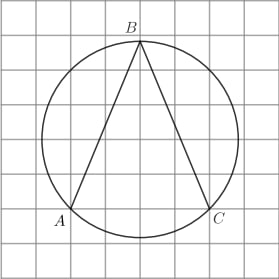
\includegraphics[align=t, width=0.3\linewidth]{\picpath/G92M7L2}
		\end{center}
		\item Найдите градусную меру дуги \( AC \) окружности, на которую опирается угол \( ABC \). Ответ
		дайте в градусах.
		\begin{center}
			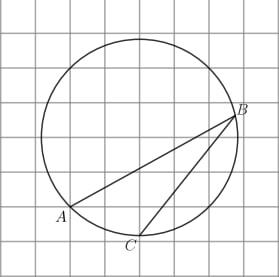
\includegraphics[align=t, width=0.3\linewidth]{\picpath/G92M7L2-2}
		\end{center}
		\item Найдите угол \( AOB \), изображенный на рисунке. Ответ дайте в градусах.
		\begin{center}
			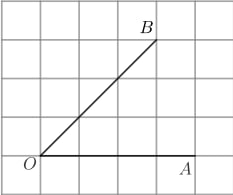
\includegraphics[align=t, width=0.3\linewidth]{\picpath/G92M7L2-3}
		\end{center}
		\item На клетчатой бумаге с размером клетки \( 1X1 \) изображён угол \( AOB \). Найдите его тангенс.
		\begin{center}
			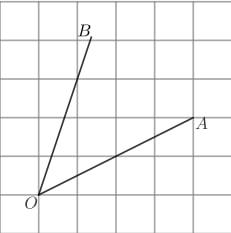
\includegraphics[align=t, width=0.3\linewidth]{\picpath/G92M7L2-4}
		\end{center}
		\item Моторная лодка прошла \( 36 \) км по течению реки и вернулась обратно, потратив на весь путь \( 5 \) часов. Скорость течения реки равна \( 3 \) км/ч. Найдите скорость лодки в неподвижной воде.
		\item Баржа прошла по течению реки \( 48 \) км и, повернув обратно, прошла ещё \( 36 \) км, затратив на весь путь \( 6 \) часов. Найдите собственную скорость баржи, если скорость течения реки равна \( 5 \) км/ч.
		\item Теплоход проходит по течению реки до пункта назначения \( 280 \) км и после стоянки возвращается в пункт отправления. Найдите скорость теплохода в неподвижной воде, если скорость течения равна \( 4 \) км/ч, стоянка длится \( 15 \) часов, а в пункт отправления теплоход возвращается через \( 39 \) часов после отплытия из него.
		\item Из пунктов \( A \) и \( B \), расстояние между которыми \( 19 \) км, вышли одновременно навстречу друг другу два пешехода и встретились в \( 9 \) км от \( A \). Найдите скорость пешехода, шедшего из \( A \), если известно, что он шёл со скоростью, на \( 1 \) км/ч большей, чем пешеход, шедший из \( B \), и сделал в пути получасовую остановку.
		\item Расстояние между городами \( A \) и \( B \) равно \( 750 \) км. Из города \( A \) в город \( B \) со скоростью \( 50 \) км/ч выехал первый автомобиль, а через три часа после этого навстречу ему из города \( B \) выехал со скоростью \( 70 \) км/ч второй автомобиль. На каком расстоянии от города \( A \) автомобили встретятся?
	\end{listofex}
\end{class}
%END_FOLD

%BEGIN_FOLD % ====>>_____ Занятие 4 _____<<====
\begin{class}[number=4]
	\begin{listofex}
		\item Занятие 4
	\end{listofex}
\end{class}
%END_FOLD

%BEGIN_FOLD % ====>>_ Домашняя работа 2 _<<====
\begin{homework}[number=2]
	\begin{listofex}
		\item Домашняя работа 2
	\end{listofex}
\end{homework}
%END_FOLD

%BEGIN_FOLD % ====>>_____ Занятие 5 _____<<====
\begin{class}[number=5]
	\begin{listofex}
		\item Занятие 5
	\end{listofex}
\end{class}
%END_FOLD

%BEGIN_FOLD % ====>>_____ Занятие 6 _____<<====
\begin{class}[number=6]
	\begin{listofex}
		\item Занятие 6
	\end{listofex}
\end{class}
%END_FOLD

%BEGIN_FOLD % ====>>_ Домашняя работа 3 _<<====
\begin{homework}[number=3]
	\begin{listofex}
		\item Домашняя работа 3
	\end{listofex}
\end{homework}
%END_FOLD

%BEGIN_FOLD % ====>>_____ Занятие 7 _____<<====
\begin{class}[number=7]
	\title{Подготовка к проверочной}
	\begin{listofex}
		\item Занятие 7
	\end{listofex}
\end{class}
%END_FOLD

=%BEGIN_FOLD % ====>>_ Проверочная работа _<<====
\begin{exam}
	\begin{listofex}
		\item Проверочная
	\end{listofex}
\end{exam}
%END_FOLD